\subsection {Session 8, Exercise 4}
\label{8f4}

\lineparagraph {Exercise}

Give a $HAM \prec s-t-HAMPATH$ Karp-reduction.

\lineparagraph {Solution}

So we need to solve $HAM$, using $s-t-HAPATH$, e.g.:

\begin{center}
    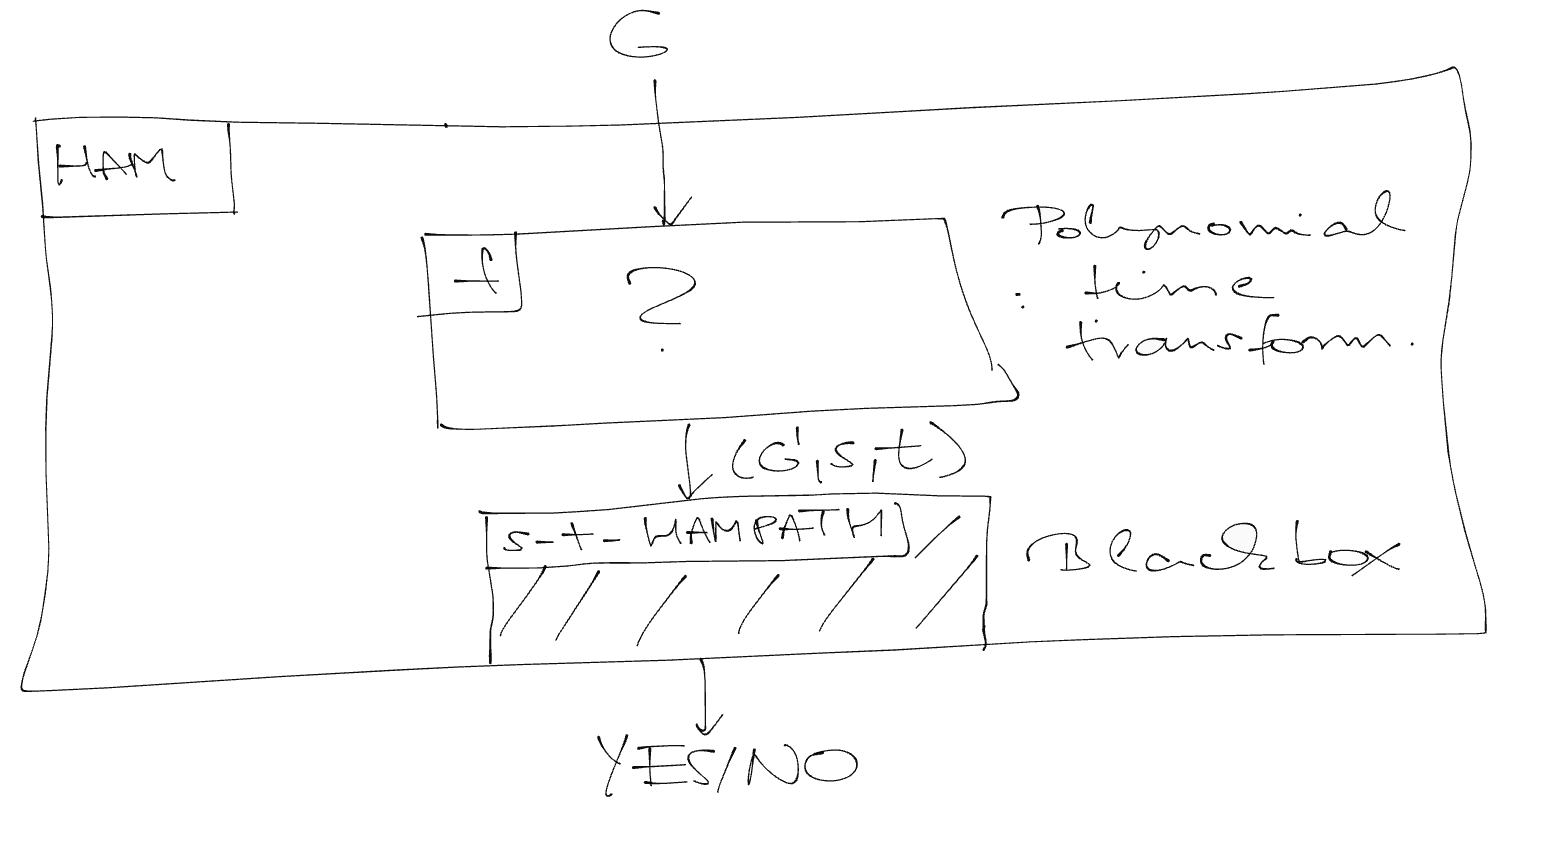
\includegraphics[width=\linewidth]{./08/03/ham_stham_karp.png}
\end{center}

\begin{itemize}
    \item The $HAM$ language gets a $G$ graph as an input and we need to transform this $G$ graph in such a way, that the $G'$ transformed graph contains an $s-t-HAMPATH$ \textbf{exactly} when the $G$ contained a Hamiltonian-cycle.
    \item The first idea that could come to mind is to just leave $G$ as is, and choose two neighbouring vertices in it, assign $s$ and $t$ to those and give these to $s-t-HAMPATH$.
    \item It is true, that if we find a Hamiltonian-path between these two vertices, then also using the fact that there is an edge between them, that edge completes the $s-t-HAMPATH$ into a Hamiltonian-cycle.
    \item However, if we do not find a Hamiltonian-path between the two vertices, then the Hamiltonian-cycle could still exist in the original graph, we might have just made an unlucky choice for $s$ and $t$. Consider the following example (the original $G$ graph is on the left, and we choose the vertices of the edge that is not part of the Hamiltonian-cycle):
\end{itemize}

\begin{center}
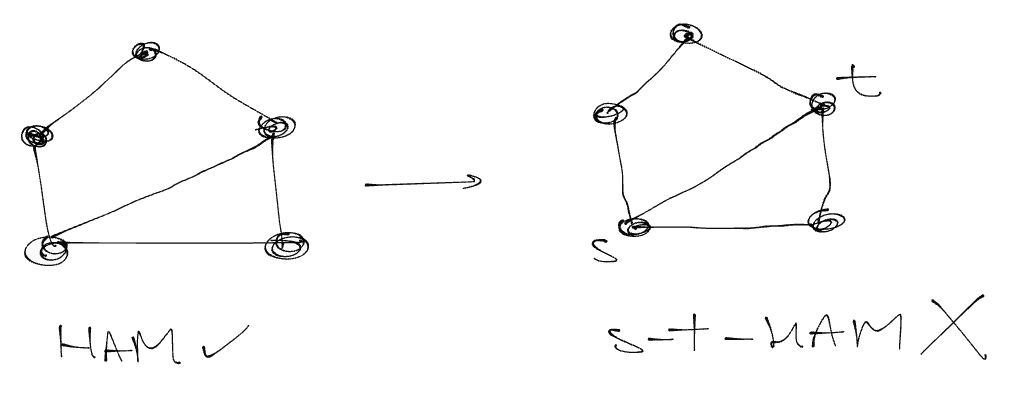
\includegraphics[width=\linewidth]{./08/03/issue_1.png}
\end{center}

\begin{itemize}
    \item The left graph has a Hamiltonian-cycle, but the right graph doesn't have an $s-t-$Hamiltonian-path.
    \item The issue here is that we tried to use different vertices and the edge between those vertices may or may not be part of the Hamiltonian-cycle.
    \item To fix, we are going to choose the same vertex twice! Well, we can't really do that, since that would contradict the definition of a path (it has to end in different vertices), but we are going to fix this by simply creating a copy of one of the vertices.
    \item So the transformation is as follows:
    \begin{itemize}
        \item Select one of the vertices of $G$, let's call this $v$.
        \item Duplicate it (add edges to the same neighbours as $v$ has) and call it $v'$.
        \item This resulting graph is $G'$, and $s=v$, $t=v'$.
        \item Give this to $s-t-HAMPATH$ and see what it returns.
    \end{itemize}
    \item If $s-t-HAMPATH$ returned a $YES$, this means that there is a Hamiltonian path between $v$ and $v'$. What does this mean in the original graph?
\end{itemize}

\begin{center}
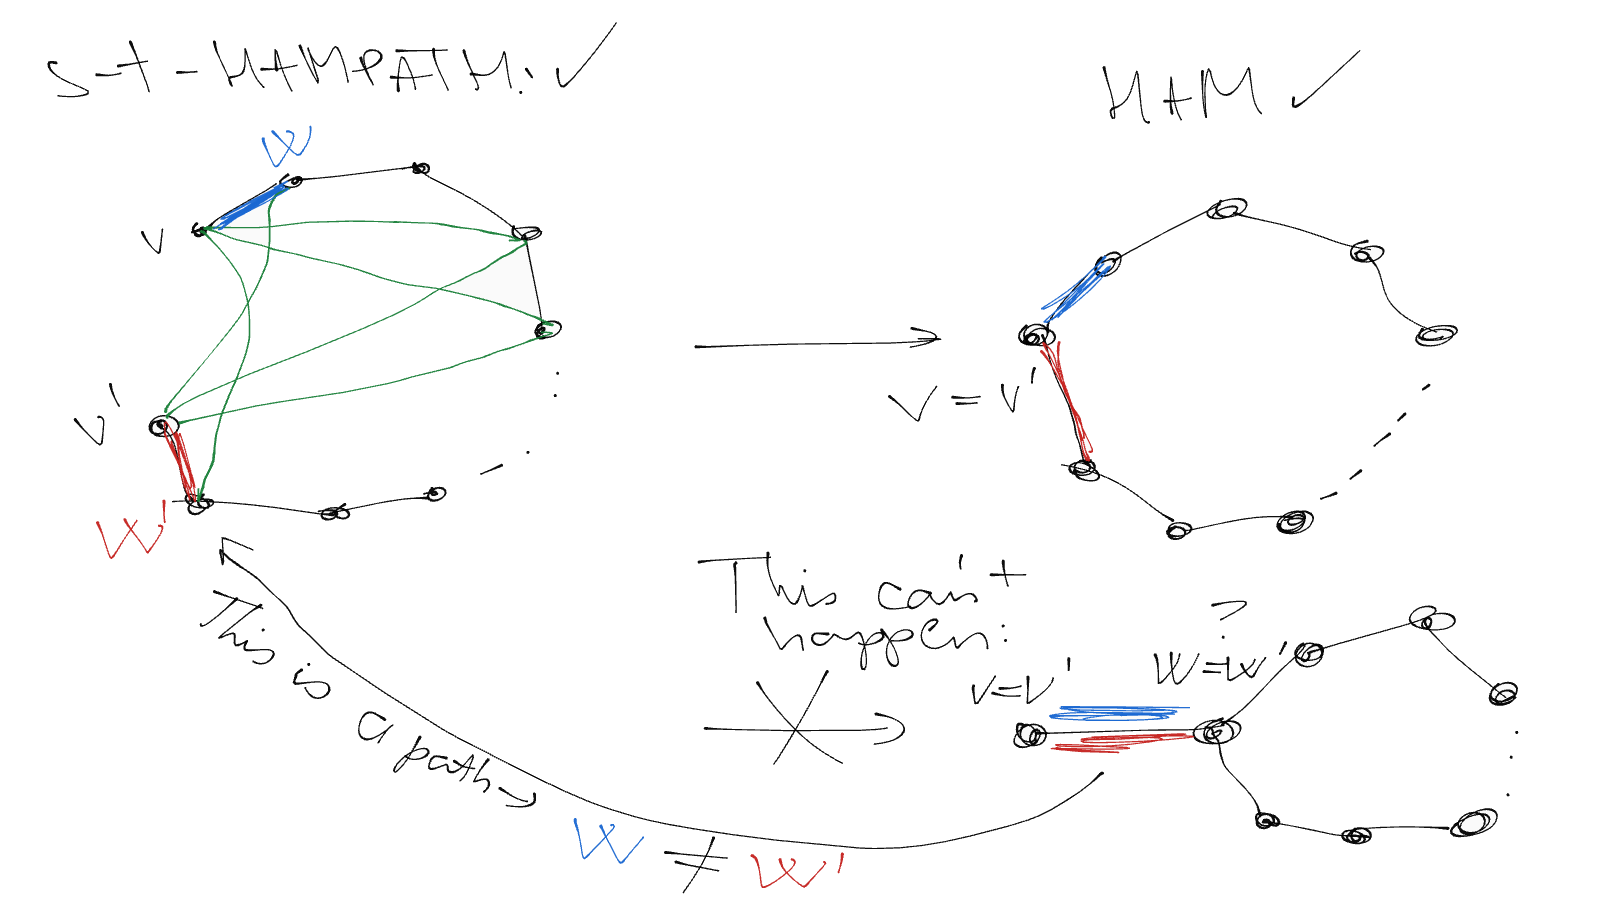
\includegraphics[width=\linewidth]{./08/03/ham_yes.png}
\end{center}

\begin{itemize}
    \item Then we can reconstruct a Hamiltonian-cycle in the original graph, as we can see on the image above.
    \item It could be an issue if the blue and the red edge were the same, because we copied $v$ to $v'$, so we might have accidentally used the same edge, however that cannot happen, because that would require $w$ and $w'$ to be the same vertex too and they cannot be, since a path cannot contain duplicate vertices.
    \item If $s-t-HAMPATH$ returned a $NO$, then this means that there cannot be a Hamiltonian-cycle in the original graph. This can be show using proof by contradiction.
    \item Let's indirectly state that $s-t-HAMPATH$ returns a $NO$, but there is a Hamiltonian-cycle in the original graph. This Hamiltonian cycle contains the $v$ vertex we duplicated, since it contains all vertices of the graph.
    \item When we duplicated the $v$ to $v'$, the Hamiltonian-cycle was broken up into a path that contains all vertices and starts in $v$ and ends in $v'$. Which means this is a $v-v'$-Hamiltonian-path, or an $s-t$-Hamiltonian path, so $s-t-HAMPATH$ could not have returned a $NO$ answer. See below:
\end{itemize}

\begin{center}
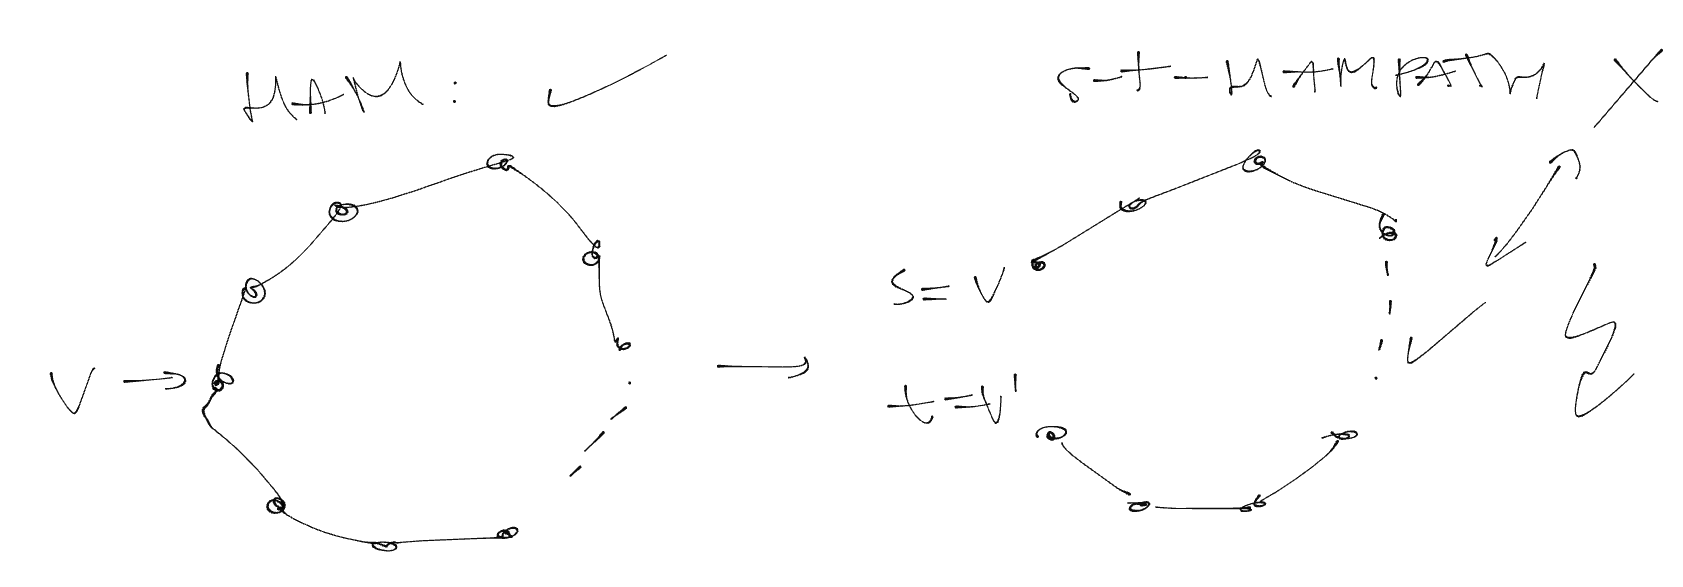
\includegraphics[width=\linewidth]{./08/03/ham_no.png}
\end{center}

\begin{itemize}
    \item This is a contradiction, so we have shown that the original statement was true, if $s-t-HAMPATH$ returned a $NO$, then this means that $HAM$ will return a $NO$ too, for $G', s, t$.
\end{itemize}